% !TEX root = main.tex
\section{Human Agreement and Additional Judge Panels}\label{app:exp16-exp17}
\subsection{Agreement between annotation passes}\label{app:human-agreement}
Table~\ref{tab:app-human-human-ceiling} reports the frozen agreement statistics on 72 shared analyzed pairs.
The passes reflect different rubric strictness levels from the same annotator, rather than independent draws from a rater population.
Their disagreement cannot identify a numerical ceiling on model agreement.
The original rubric text remains unavailable.

\begin{table}[H]
\centering\small
\begin{tabular}{@{}lrc@{}}
\toprule
Statistic & Estimate & 95\% bootstrap interval \\
\midrule
Spearman correlation & 0.249 & $[-0.015,0.489]$ \\
Pearson correlation & 0.375 & $[0.076,0.604]$ \\
Kendall correlation & 0.221 & $[-0.016,0.442]$ \\
Quadratic-weighted $\kappa$ & 0.372 & $[0.073,0.581]$ \\
Mean absolute error & 0.771 & Not reported \\
\bottomrule
\end{tabular}
\caption{The two human passes disagree on the same artifacts, making the choice of label view consequential.
Mean absolute error uses the original $0$--$5$ rating scale; all estimates use 72 overlapping pairs.}
\label{tab:app-human-human-ceiling}
\end{table}

\subsection{Expanded configuration panel}\label{app:expanded-panel}
The expanded panel compares the arithmetic $v2$ with the pass1-selected geometric form $\mathrm{mono}^{0.4}\mathrm{stab}^{0.6}$.
Its averaged-label association is $0.769$, with bootstrap interval $[0.34,0.95]$ (Figure~\ref{fig:app-exp25-13judge}).
The result concerns 13 configurations on reused validation labels, not 13 independent model families or unseen data.
The plotted geometric index is not $\mathrm{TI}_{\mathrm{var}}$.

\begin{figure}[htbp]
\centering
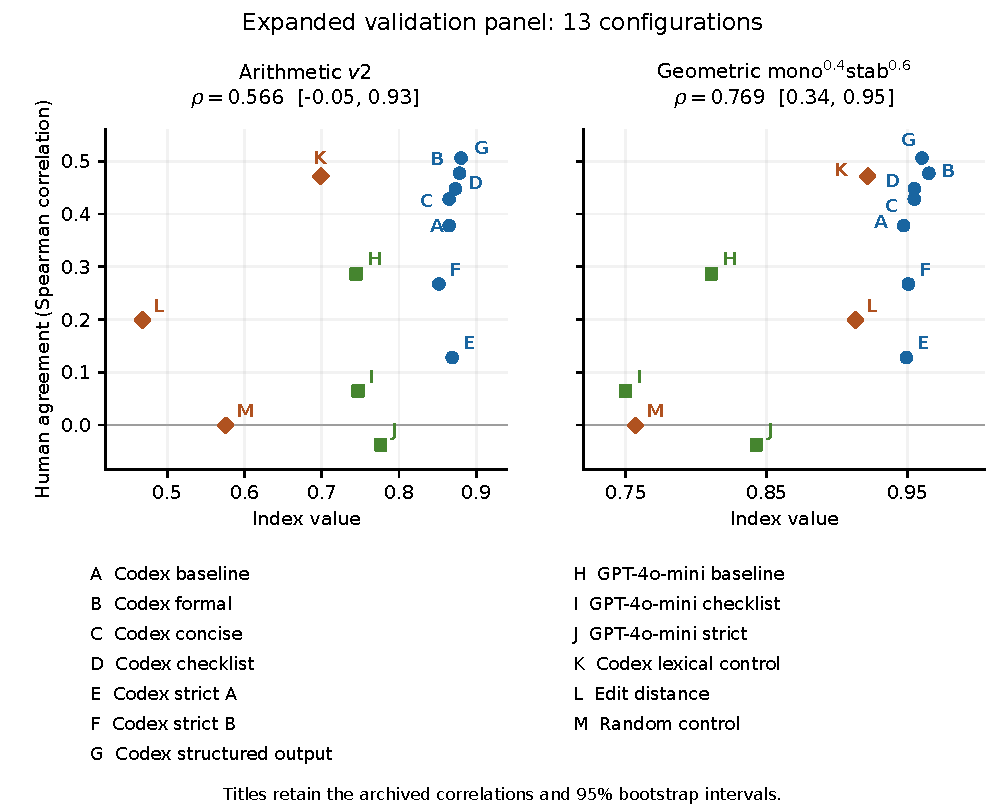
\includegraphics[width=\linewidth]{figures/expanded_panel_v2_vs_geometric.pdf}
\caption{The tuned geometric comparison has a positive association on the expanded validation panel.
The two panels compare arithmetic $v2$ with $\mathrm{mono}^{0.4}\mathrm{stab}^{0.6}$ across 13 configurations; the figure retains the archived estimates and intervals.}
\label{fig:app-exp25-13judge}
\end{figure}

\subsection{Negative results}\label{app:negative-results}
A separate Leanstral panel yields $\mathrm{TI}_{\mathrm{var}}$ associations of $-0.1190$, $-0.0476$, and $-0.0952$ on pass1, pass2, and averaged labels.
It uses \texttt{labs-leanstral-2603} in the same eight-configuration form, with three recorded scores per row for every configuration and median aggregation.
Its five-configuration semantic subset remains negatively associated on all three label views (Table~\ref{tab:subset-diagnostics}).
These recorded results contradict a claim that the fixed index works for every family.
They do not establish why the association fails.
The different-rubric human pool described in Section~\ref{sec:limitations-test} also produced no qualifying index in either registered screen.
The 32-configuration screen's largest absolute association is negative, so its sign does not support the proposed direction of the screen even before accounting for multiple comparisons.

\subsection{Can model raters substitute for human raters?}\label{app:model-raters-substitution}
Human ratings are the binding cost in judge validation, so a natural scaling route is to let frontier models stand in for the human raters and validate the judge against them.
We report a direct test of that route, run on VeriBench VBV1 (experiment 106), because the result bears on any attempt to scale judge validation without additional human ratings.
The motivating obstacle is that the available human ratings cover a single agent, so they cannot answer whether a judge generalizes to agents it has not seen.

\paragraph{Design.}
Seven frontier models, one per model family, each rate the same artifacts under the human rating instructions, both as personas constructed from the expert raters' own scores and from the instructions alone.
Their aggregate is the stand-in panel.
A judge is then validated leave-one-agent-out across fourteen agent groups of fifty tasks each: one group is held out, and agreement with the panel is measured on it.
Three judge arms are compared: the frozen deployed judge, a bare-instruction judge, and a judge rebuilt from scratch on every fold.
Against the panel the frozen judge reaches pooled Spearman $0.917$ $[0.888, 0.937]$ with $\mathrm{ICC}(A,1)$ $0.922$, which taken alone would read as strong evidence of generalization.

\paragraph{The anchor.}
One held-out group consists of exactly the items the expert raters scored, so on that group every judge can be measured against the stand-in panel and against the human raters on identical items.
Table~\ref{tab:app-standin-vs-human} reports both.

\begin{table}[H]
\centering\small
\begin{tabular}{@{}lcc@{}}
\toprule
Judge & vs.\ stand-in panel & vs.\ human raters \\
\midrule
Frozen deployed judge & $0.82$ & $0.772$ $[0.570, 0.901]$ \\
Rebuilt per fold & $0.91$ & $0.621$ $[0.278, 0.832]$ \\
Bare instructions & $0.86$ & $0.563$ $[0.176, 0.806]$ \\
\bottomrule
\end{tabular}
\caption{Spearman agreement of three judges on one held-out group of $75$ items, measured against the model stand-in panel and against the human raters who scored those same items.}
\label{tab:app-standin-vs-human}
\end{table}

\paragraph{Why substitution fails here.}
The panel agrees with the human raters at Spearman $0.770$ $[0.527, 0.898]$, and the judge it is grading agrees with those same raters at $0.772$ $[0.570, 0.901]$.
The substitute is therefore no more accurate than the instrument it is being used to assess, and agreement measured against it cannot separate judge quality from error the two share.
The inflation is largest for the judge that was itself built against the panel, whose agreement falls from $0.91$ to $0.621$, roughly twice the drop of the judge that was not.
Fitting a judge to model raters fits their idiosyncrasies.
Raising panel quality did not remove the problem.
Constructing the stand-in raters from the expert raters' own scores added nothing measurable over the rating instructions alone at the single-model stage, a paired difference of $-0.001$ $[-0.118, 0.109]$.
Widening the panel from one model to seven families raised its agreement with the human raters from $0.626$ to $0.770$, which only drew level with the judge.

\paragraph{What the substitute still supports.}
The failure is in the absolute level rather than in every comparison.
Pooled across the thirteen held-out agents the panel orders the three judge arms as $0.917$, $0.915$, and $0.876$ for the frozen, bare-instruction, and rebuilt arms, which selects the frozen judge and rejects the rebuilt one; the human evidence on the anchor group supports the same choice.
Differential quantities in which both arms carry the same shared error also survive: no judge or rater in this design favored its own model family by $0.05$ or more after Holm correction, with largest absolute effect $0.043$.
We therefore read model stand-ins as admissible for relative comparisons between judges and for same-family screens, and inadmissible as the reference for any reported judge--human agreement number.

\paragraph{Limits of this test.}
Human ratings exist for one agent group of $75$ items, so the per-judge ordering against human raters rests on point estimates whose intervals overlap.
A pre-registered non-inferiority comparison between the fold-built judge and an earlier out-of-fold judge was inconclusive, with difference $0.018$ $[-0.295, 0.338]$, rather than a refutation.
The direction is consistent across both the persona and instruction-only panels, but the single anchor group is itself the reason additional human ratings remain the binding requirement.
